\subsection{Rezonansowa transmisja przez grube siatki}
\label{subart:rezo-grating}

\begin{figure}[tb]
	\centering
	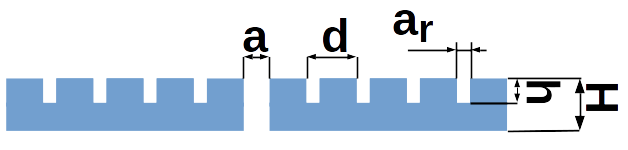
\includegraphics[width=0.9\textwidth]{images/thz/schemat-1szczelina.png}
	\caption{Schemat szczeliny otoczonej siatką rowków w celu umożliwiającej wysoką transmisję rezonansową}
	\label{fig:szczelina-schem}
\end{figure}

\begin{figure}[bt]
	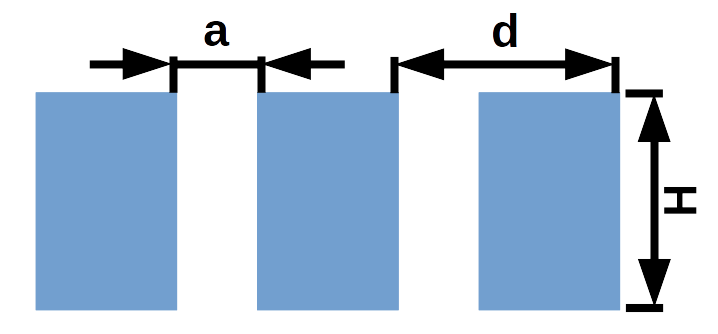
\includegraphics[width=\textwidth]{images/thz/schemat-siatka.png}
	\caption{Schemat siatki dyfrakcyjnej wykorzystywanej w symulacjach}
	\label{fig:rezo-siat-H}
\end{figure}

Modelowym układem, w którym można przeprowadzić analizę zjawisk związanych z rezonansową transmisją fali elektromagnetycznej przez siatkę z idealnego przewodnika jest układ przedstawiony na rysunku \ref{fig:szczelina-schem} oświetlony od strony rowków. Zakładając, że zarówno rowki jak i szczelina są na tyle cienkie, że możliwe jest wzbudzenie w nich jedynie modu podstawowego\footnote{Dla falowodów planarnych metal-izolator-metal nie istnieje długość fali odcięcia dla modu podstawowego w polaryzacji TM}, problem propagacji fali E-M przez układ można rozwiązać analitycznie. W tym celu promieniowanie w przestrzeni swobodnej możemy rozłożyć na fale płaskie, a wzbudzenia wewnątrz rowków i falowodu zastąpić polami modów podstawowych. Wymagając odpowiednich warunków zszycia rozwiązań nadzwyczajną transmisję~(przewyższającą o kilka rzędów wielkości transmisję przewidywaną przy pomocy rachunku opartego o współczynnik wypełnienia) przez szczelinę możemy opisać przy pomocy następujących mechanizmów~\cite{martin2001theory}:
\begin{itemize}
	\item Rezonansowa transmisja przez mod falowodowy w szczelinie. Kontrolowana przez grubość metalu $H$ na zasadzie rezonansu Fabry-P\'{e}rot. Maksimum transmisji występuje w przyjętym przybliżeniu dla
\begin{equation}
\frac{\lambda}{n_{\textrm{eff}}} = 2 \frac {H}{m},
\label{eq:fp-szczelina}
\end{equation}
gdzie $\lambda$ oznacza długość fali promieniowania padającego na układ, $H$ zgodnie z rysunkiem \ref{fig:szczelina-schem} jest długością falowodu, $m$ dowolną liczbą naturalną, a $n_{\textrm{eff}}$ efektywnym współczynnikiem załamania modu falowodowego. W przypadku falowodów metal-powietrze-metal $n_{\textrm{eff}} \approx 1$.
	\item Wzbudzenie modów w rowkach, pozwalające na późniejszy transport energii z rowków do szczeliny przy pomocy fali powierzchniowej. Dzięki temu mechanizmowi transmisja przez szczelinę unormowana do rozmiarów otworu może być znacznie większa od 1. Warunek na rezonansowe wzbudzenie modów wewnątrz szczelin to $\lambda \approx 4 \frac {h}{2m+1}$ (patrz rys. \ref{fig:szczelina-schem}, wykorzystanie tego wzbudzenia możliwe jest jednak jedynie przy dopasowanej reemisji energii z kolejnych rowków.
	\item Zgodne w fazie drgania modów w rowkach, pozwalające na wzbudzenie w płaszczyźnie wejściowej fali powierzchniowej transportującej energię fali E-M do szczeliny. Sytuacja taka występuje dla $d \approx \lambda$.
\end{itemize}

Należy podkreślić, że w używanym modelu pominięto wpływ fal ewanescętnych, jest to uprawnione dla przewidywania transmisji przez strukturę w polu dalekim ze względu na eksponencjalny zanik tych modów wraz z odległością od warstwy metalowej. Jednakże należy mieć świadomość, że obecne w okolicach struktury fale ewanescętne mają istotny wpływ na wymienione mechanizmy~\cite{ebbesen1998extraordinary}.

Przeprowadzona analiza teoretyczna opisuje jedynie mechanizmy prowadzące do nadzwyczajnej transmisji przez szczelinę otoczoną rowkami w przypadku układu jednowymiarowego. Przewidywania płynące z opisanych wyżej zjawisk fizycznych zostały jednak poddane weryfikacji z wynikami eksperymentalnymi dotyczącymi układów dwuwymiarowych z otworami cylindrycznymi~\cite{ebbesen1998extraordinary} i prostokątnymi~\cite{koerkamp2004strong}, wykazując możliwość uogólnienia przedstawionego modelu.

\begin{figure}[tb]
\begin{subfigure}{0.45\textwidth}
	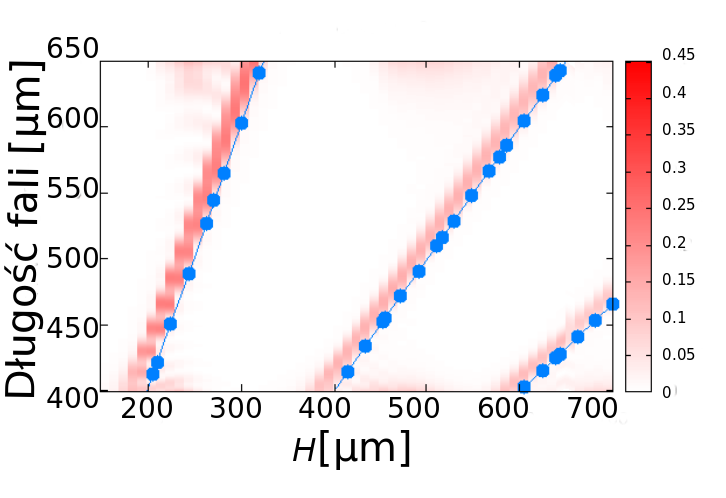
\includegraphics[width=\textwidth]{images/antenaThz/rezonant_trans_f001.png}
	\caption{$f=$99\%,~d=400~$\mu$m }
	\label{fig:rezof001}
\end{subfigure}
\begin{subfigure}{0.45\textwidth}
	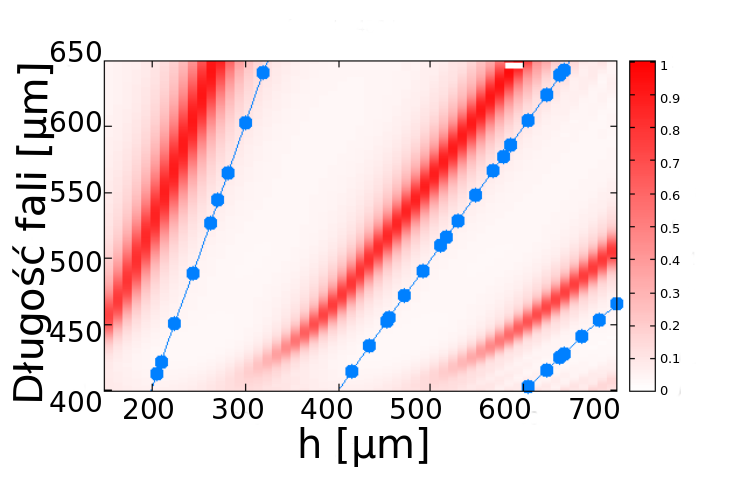
\includegraphics[width=\textwidth]{images/antenaThz/rezonant_trans_f01.png}
	\caption{$f=$90\%,~d=400~$\mu$m }
	\label{fig:rezof01}
\end{subfigure}

\begin{subfigure}{0.45\textwidth}
	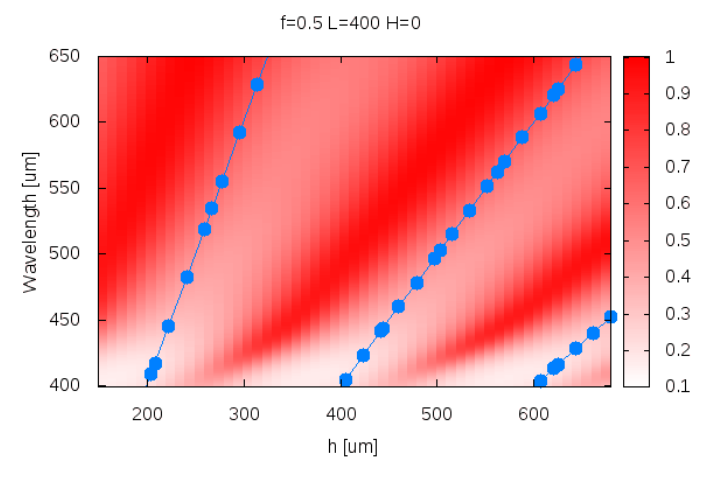
\includegraphics[width=\textwidth]{images/antenaThz/rezonant_trans_f05.png}
	\caption{$f=$50\%,~d=400~$\mu$m }
	\label{fig:rezof05}
\end{subfigure}
\begin{subfigure}{0.45\textwidth}
	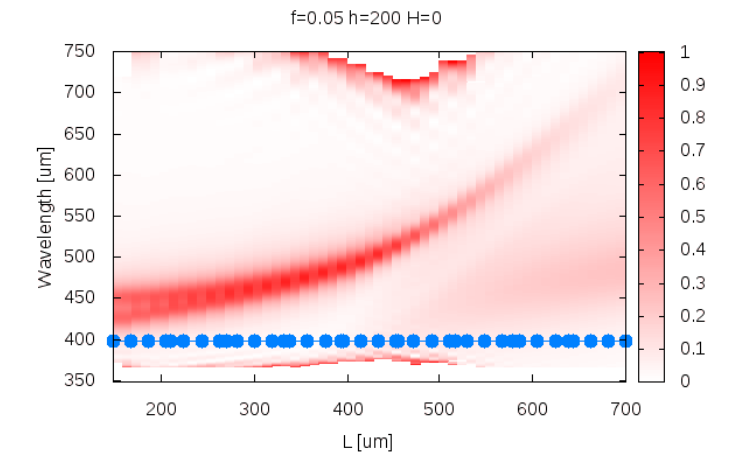
\includegraphics[width=\textwidth]{images/antenaThz/rez_trans_L.png}
	\caption{$f=$90\%,~H=400~$\mu$m}
	\label{fig:rezL}
\end{subfigure}

\caption{Zależność współczynnika transmisji od parametrów geometrycznych siatki. Niebieską linią kropkowaną zaznaczono przewidywane wzorem (\ref{eq:fp-szczelina}) położenie maksimum rezonansu transmisji. }
\label{fig:rezo-siat-H}
\end{figure}

Ze względu na trudności w eksperymentalnej realizacji układu z rysunku \ref{fig:szczelina-schem}, oraz zależności położenia od rezonansu (\ref{eq:fp-szczelina}) jedynie od grubości w kolejnych symulacjach skupiono się na siatce dyfrakcyjnej jak na rysunku \ref{fig:rezo-siat-H}.  Za pomocą symulacji metodą FDTD sprawdzono przewidywane w przybliżeniu cienkich falowodów położenie rezonansu, oraz dokonano ilościowego oszacowania transmisji promieniowania THz przez nieskończoną jednowymiarową metalową siatkę dyfrakcyjną w zależności od jej grubości $H$ i współczynnika wypełnienia $f=\frac{a}{d}$. Wykresy przedstawione na rysunku \ref{fig:rezo-siat-H} wykazują, że nawet dla siatek dyfrakcyjnych o szerokich, chociaż ciągle znacząco podfalowych otworach, jak $a=40$~$\mu$m możliwe jest uzyskanie transmisji rezonansowej. Położenie rezonansu ulega jednak przesunięciu w kierunku większych długości fali \cite{Szczytko2012271}.

Za pomocą symulacji metodą FDTD wykazano również, że wraz ze wzrostem okresu siatki $d$ następuje zarówno przesunięcie maksimum rezonansu w kierunku dłuższych fal, jak i zawężenie transmitowanego pasma. Wydłużenie okresu siatki może więc posłużyć do zawężenia zakresu transmitowanych długości fali przy jednoczesnym powiększeniu otworów. Rozkład energii całkowitej pola E-M uzyskiwanego przy oświetleniu omawianych siatek złotych falą o długości znajdującej się w maksimum transmisji przedstawia rysunek \ref{fig:consrcl525}, natomiast rozkład pola powstający w przypadku źródła odstrojonego od rezonansu przedstawia rysunek \ref{fig:consrcl500}.

\begin{figure}[bth]
	\begin{subfigure}{0.45\textwidth}
		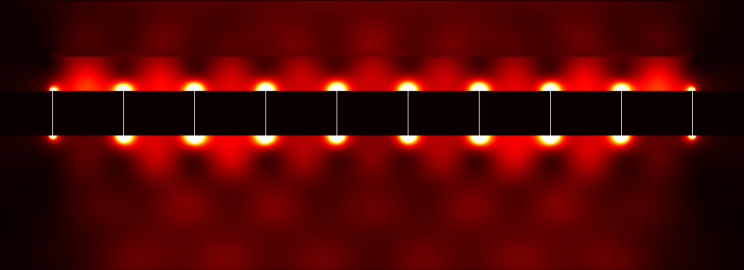
\includegraphics[width=\textwidth]{images/thz/con_src_l525.png}
		\caption{$H=$250~$\mu$m, $\lambda=$525~$\mu$m}
		\label{fig:consrcl525}
	\end{subfigure}
	\begin{subfigure}{0.45\textwidth}
		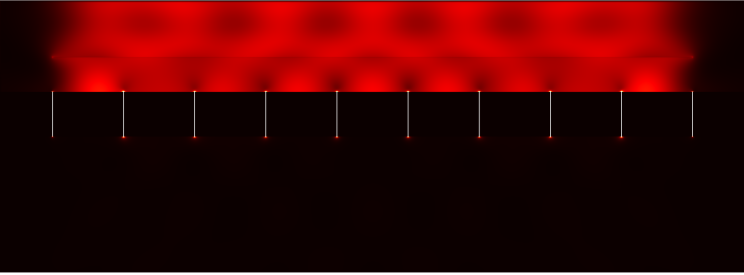
\includegraphics[width=\textwidth]{images/thz/con_src_l500.png}
		\caption{$H=$250~$\mu$m, $\lambda=$500~$\mu$m}
		\label{fig:consrcl500}
	\end{subfigure}
	\caption{Rozkład całkowitej energii pola E-M dookoła siatki złotej oświetlonej z góry za pomocą monochromatycznego źródła o długości fali $\lambda$} 
\end{figure}

